\newpage % Rozdziały zaczynamy od nowej strony.
\cleardoublepage % Zaczynamy od nieparzystej strony
\pagestyle{headings}

\section{Wyniki i wnioski}

Celem pracy było zaprojektowanie, nauczenie i przetestowanie działania algorytmu Sztucznej Sieci Neurnonowej z użyciem 
układu FPGA oraz porównanie z rozwiązaniem programowym. Podczas projektu powstało kilka modeli Sztucznej Sieci 
Neuronowej klasyfikującej odręcznie pisane cyfry. Aby porównać rozwiązanie, realizowane w technice HLS z implementacją 
przy użyciu pakietu \emph{keras}, każdy z modeli poddano testom, które zostały podzielone na dwie części:
\bigskip
\begin{enumerate}
  \item Uruchomienie sieci przy użyciu zbioru testowego 10000 cyfr z bazy MNIST, w celu oszacowania dokładności i 
  szybkości działania algorytmu.
  \item Test wykonany w czasie rzeczywistym przy użyciu modułu kamery.
\end{enumerate}

Wyniki przeprowadzonych testów zostały zestawione w dalszej części rozdziału.

\subsection{Test modelu sieci z jedną warstwą ukrytą}

Wykonano test, podając na wejście sieci 10000 obrazów. Wynik testu, widoczny na Rys. \ref{wynik1} potwierdził poprawność działania algorytmu. Osiągnięto dokładność na poziomie 94,97\%, co pokrywa się z wynikiem uzyskanym z wykorzystaniem biblioteki \emph{keras}.

\begin{figure}[!h]
    \centering
    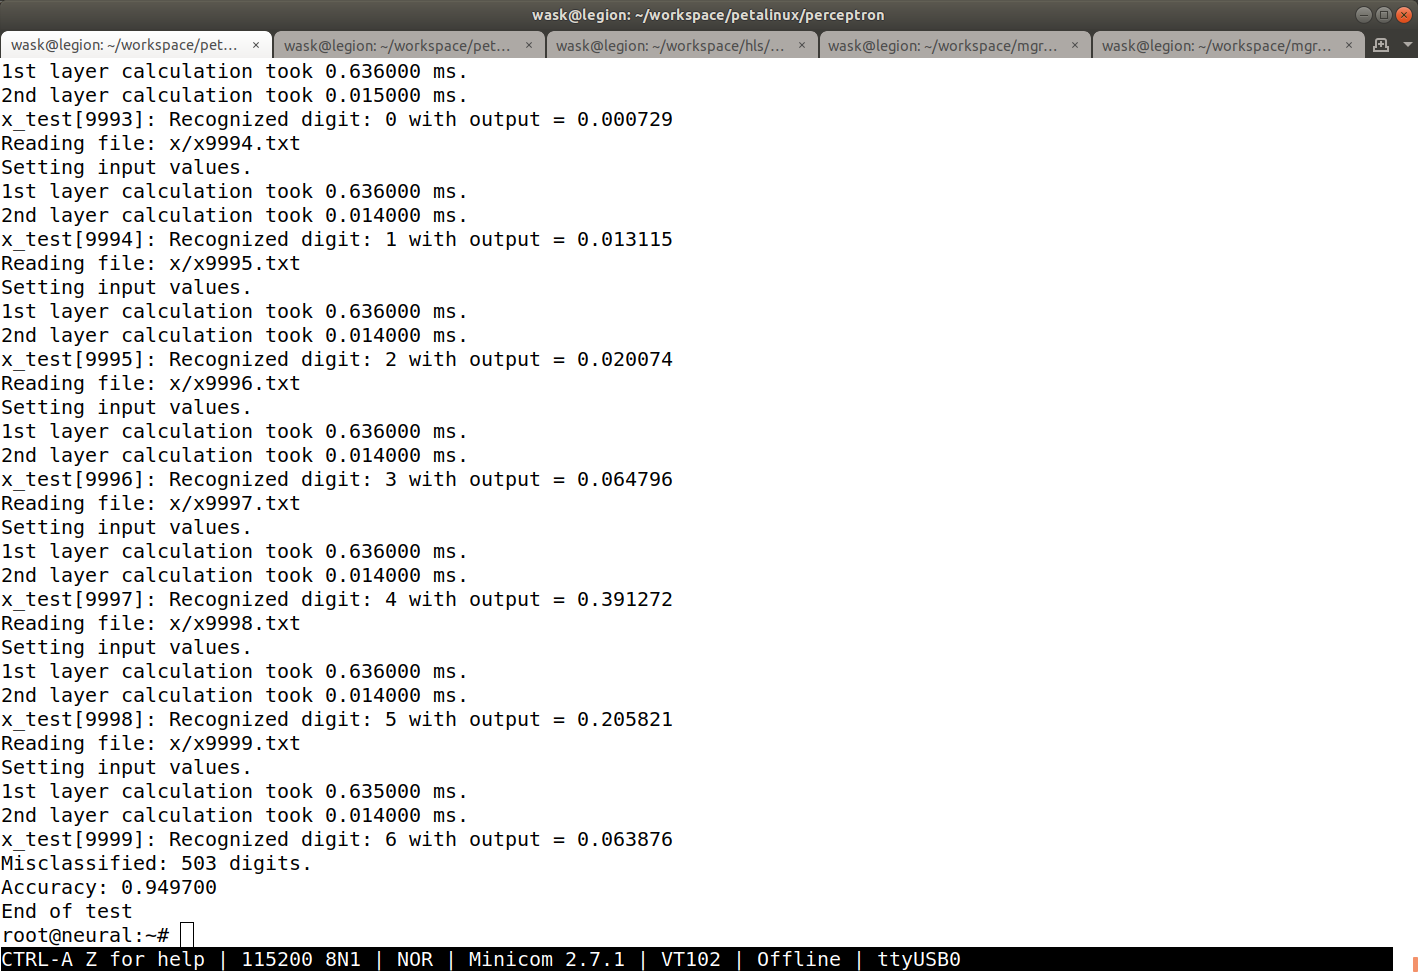
\includegraphics[width=\textwidth]{img/wynik1.png}
    \caption{Wynik testu uruchomionego na SBC Z-turn -- ANN z jedną warstwą ukrytą}
    \label{wynik1}
  \end{figure}


\subsubsection{Test klasyfikacji cyfr z użyciem kamery}

Następnym krokiem był test przeprowadzony w czasie rzeczywistym z użyciem kamery. Rozpoznawanie obiektów na obrazie w czasie rzeczywistym podzielono na 3 części:
\begin{itemize}
    \item detekcja kształtów przypominających cyfry i odrzucenie niewłaściwych obiektów
    \item przygotowanie obrazów do klasyfikacji (odpowiedni rozmiar obrazu i padding)
    \item klasyfikacja obrazów przy użyciu ANN
\end{itemize}

Pierwszą symulację wykonano na komputerze PC przy użyciu biblioteki OpenCV i pakietu \emph{keras}.
Ze względu na sporą ilość obliczeń początkowo zdecydowano się na zarejestrowanie obrazu oraz detekcję cyfr przy użyciu biblioteki OpenCV. 

Obraz był rejestrowany w rozdzielczości 640x480 pikseli przy użyciu funkcji  \emph{cv2.VideoCapture(2)}. Następnym krokiem było przekształcenie barwy obrazu na skalę szarości, rozmycie obrazu oraz za pomocą funkcji \emph{cv2.adaptiveThreshold} przekształcenie w obraz binarny. Następnie użyto funkcji \emph{cv2.findContours}, która zwraca współrzędne prostokątów, w które wpisane są kontury znalezione przez algorytm. Po wyeliminowaniu niewłaściwych konturów można przejść do przygotowania obrazów do klasyfikacji. 

\begin{figure}[!h]
    \centering
    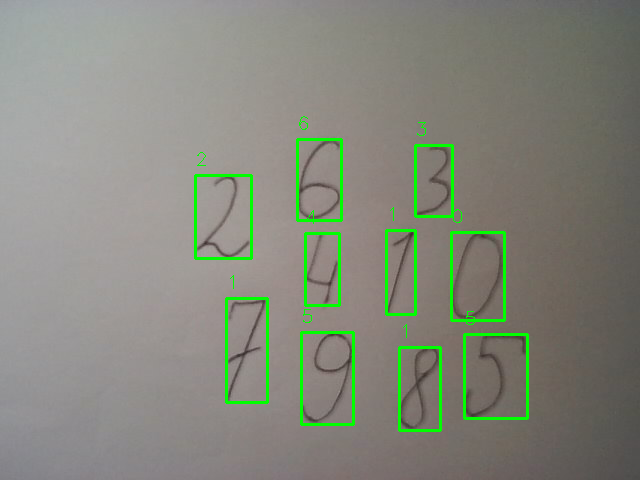
\includegraphics[width=\textwidth]{img/1hid-layer-pc-img.png}
    \caption{Ramka obrazu podczas testu ANN z jedną warstwą ukrytą uruchomionego na PC}
    \label{1hid-layer-pc-img}
  \end{figure}

Odpowiednio przycięty do rozmiaru 28x28 pikseli i wycentrowany obraz ręcznie pisanej cyfry może zostać poddany klasyfikacji za pomocą nauczonego wcześniej modelu ANN. W wyniku testu otrzymano wyniki przedstawione na Rys. \ref{1hid-layer-pc-img}. 

\begin{figure}[!h]
    \centering
    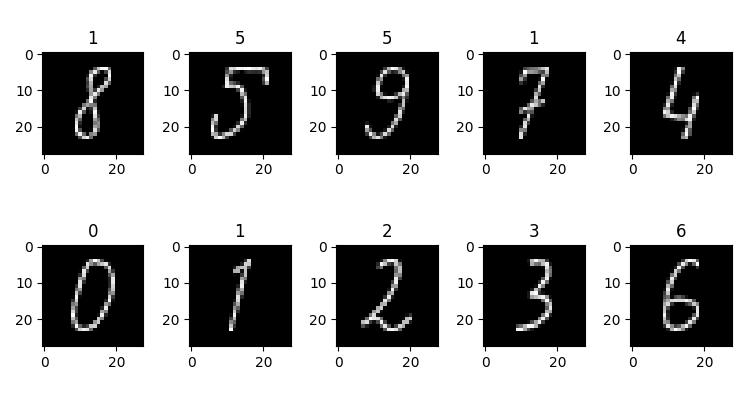
\includegraphics[width=\textwidth]{img/1hid-layer-pc-plot.png}
    \caption{Wynik testu ANN z jedną warstwą ukrytą uruchomionego na PC}
    \label{1hid-layer-pc-plot}
\end{figure}


Rysunek Rys. \ref{1hid-layer-pc-plot} zawiera znalezione na obrazie cyfry i wynik klasyfikacji (nad każdą z cyfr). Widać, że 3 z 10 cyfr zostały sklasyfikowane nieprawidłowo, co daje dokładność klasyfikacji sieci 70\%.

\subsubsection{Test na płytce Z-turn z użyciem kamery}

W teście na płytce Z-turn zastosowano metodę rejestrowania obrazu taką jak na komputerze PC, jednak do rozpoznania cyfr wykorzystano model sieci ANN zaimplementowany w układzie FPGA. Aby umożliwić użytkownikowi wyświetlanie obrazu w czasie rzeczywistym, wykorzystano pakiety \emph{pickle} i \emph{socket} do wysyłania kolejnych ramek obrazu przez protokół TCP (ang. \emph{Transmission Control Protocol}). Wynik testu przedstawiono na Rys. \ref{1hid-layer-zturn-img}.

\begin{figure}[!h]
    \centering
    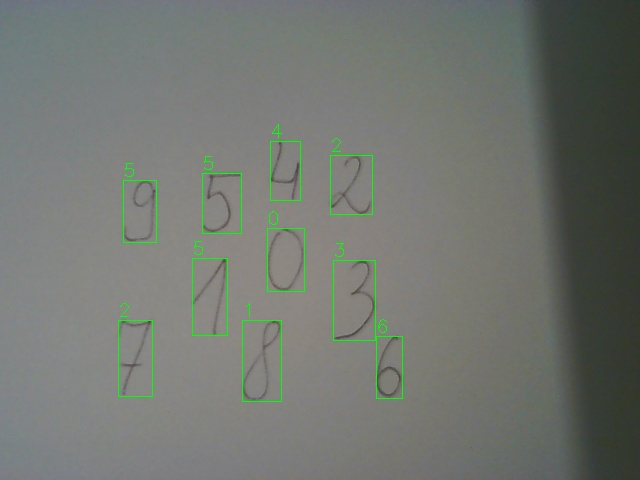
\includegraphics[width=\textwidth]{img/1hid-layer-zturn-img.jpg}
    \caption{Wynik testu ANN z jedną warstwą ukrytą uruchomionego na płytce Z-turn Board}
    \label{1hid-layer-zturn-img}
\end{figure}

Po otrzymaniu wyników pierwszego testu podjęto decyzję o modyfikacji modelu Sztucznej Sieci Neuronowej. Pierwszą zmianą było dodanie kolejnej warstwy ukrytej.

\subsection{Test modelu posiadającego dwie warstwy ukryte}

Dodano do itniejącego modelu kolejną warstwę ukrytą zawierającą 64 neurony. Po wykonaniu 50 epok otrzymano dokładność na poziomie 97,17\%. Wykres zmiany dokładności w kolejnych epokach przedstawiono na Rys. \ref{keras-accuracy2}.

\begin{figure}
    \centering
    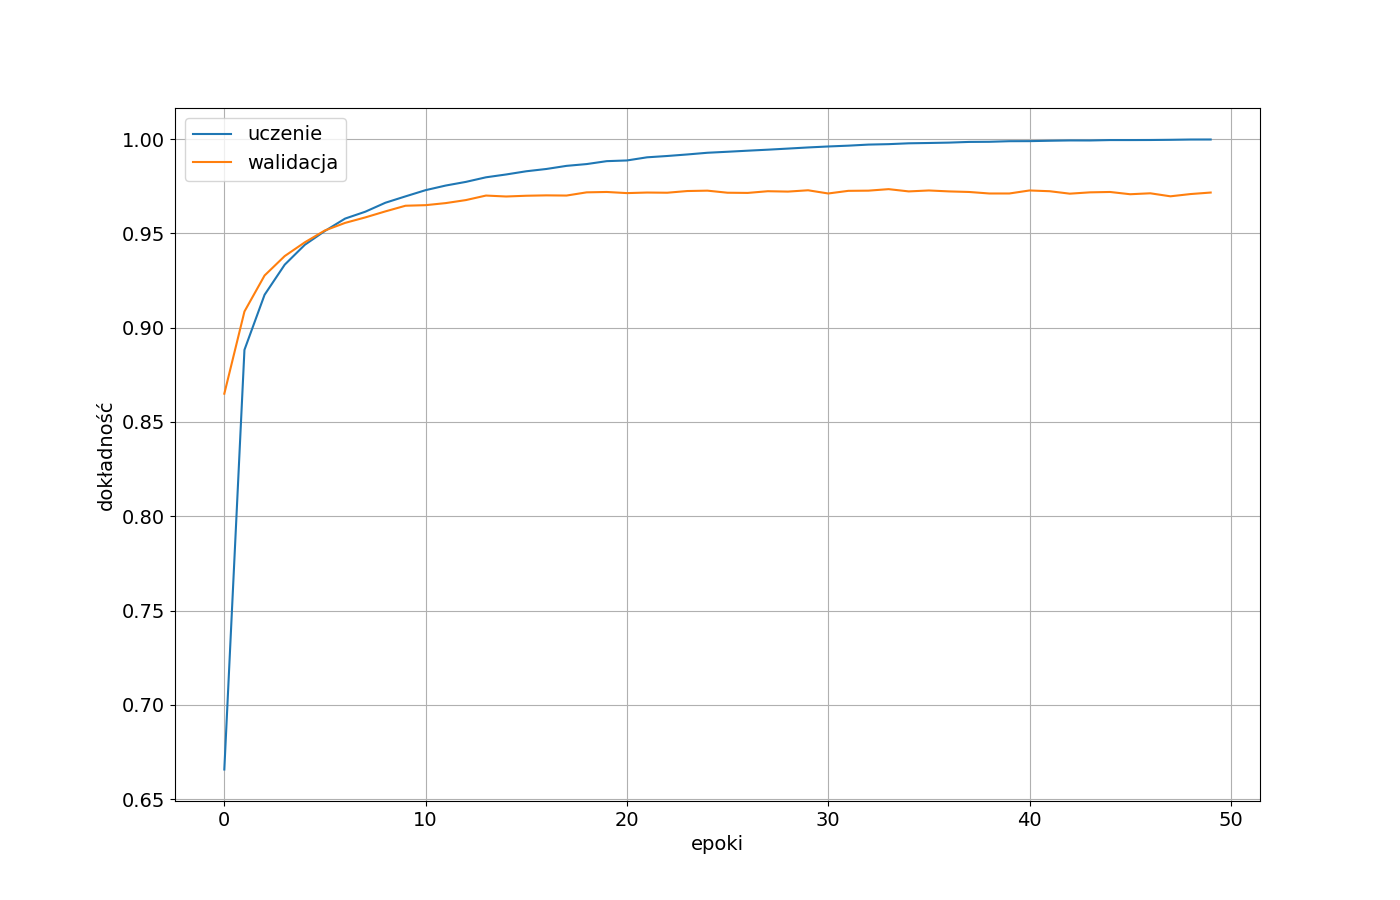
\includegraphics[width=\textwidth]{img/keras-accuracy2.png}
    \caption{Wykres zmian dokładności w kolejnych epokach -- ANN z dwoma warstwami ukrytymi}
    \label{keras-accuracy2}
  \end{figure}


